\documentclass[a4paper,12pt]{article}
\usepackage{parskip}
\usepackage{graphicx}
\usepackage{float}

\begin{document}
It is essential to include the \texttt{graphicx} and \texttt{float} packages when inserting images.

The image below sets the width to be 90\% of the width of the text:
\begin{figure}[H]
  \centering
  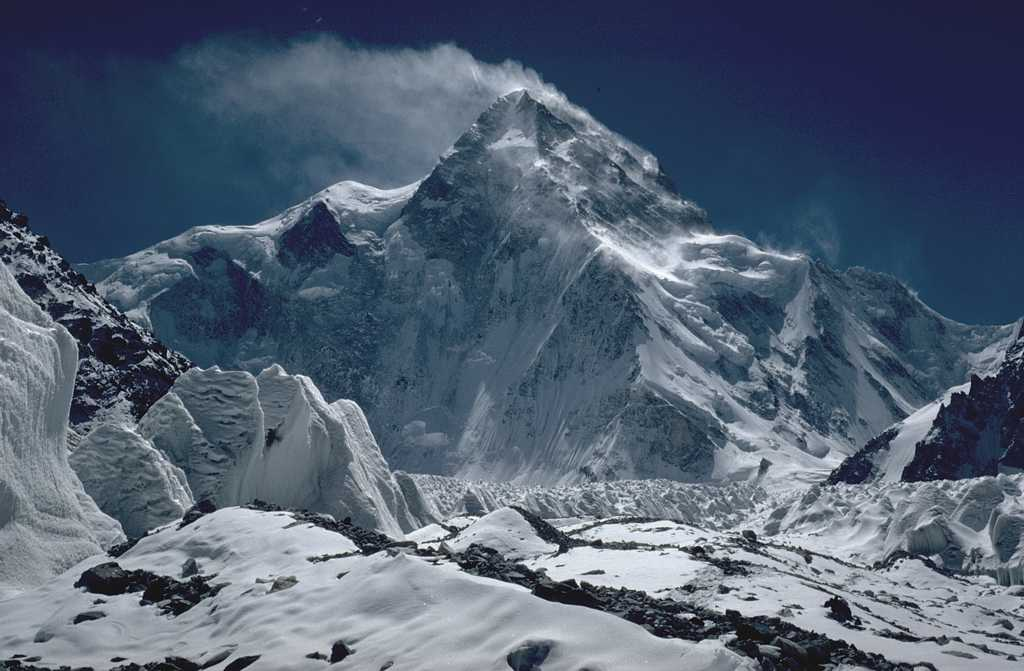
\includegraphics[width=0.9\textwidth]{k2.jpg}
  \caption{The K2 mountain in Baltistan}
\end{figure}

The image below sets the width to be 50mm:
\begin{figure}[H]
  \centering
  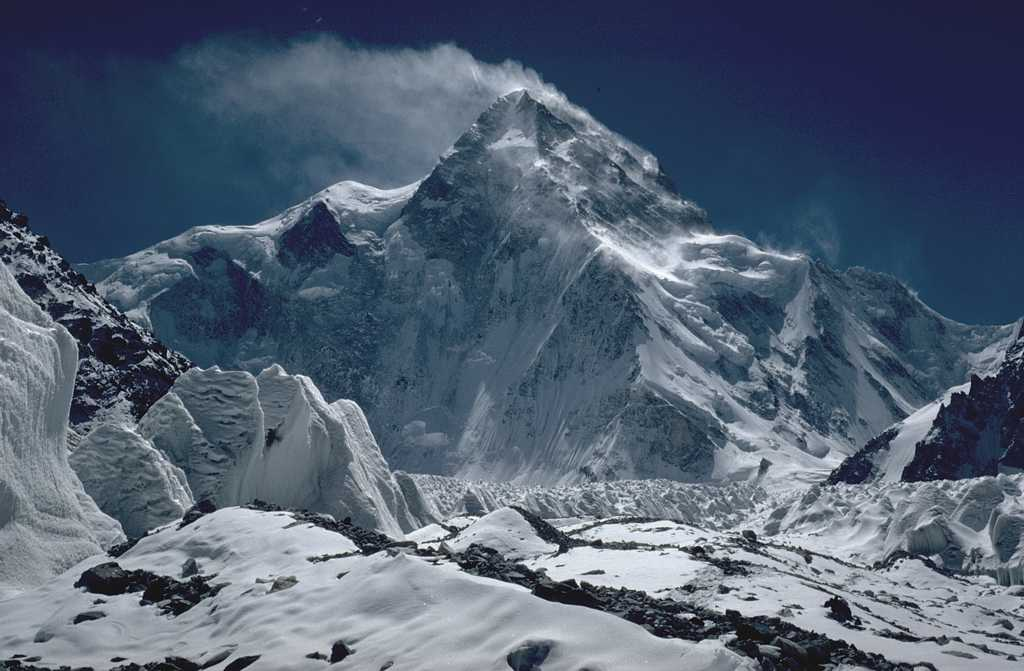
\includegraphics[width=50mm]{k2.jpg}
  \caption{The K2 mountain in Baltistan}
\end{figure}

The image below sets the height to be 10mm:
\begin{figure}[H]
  \centering
  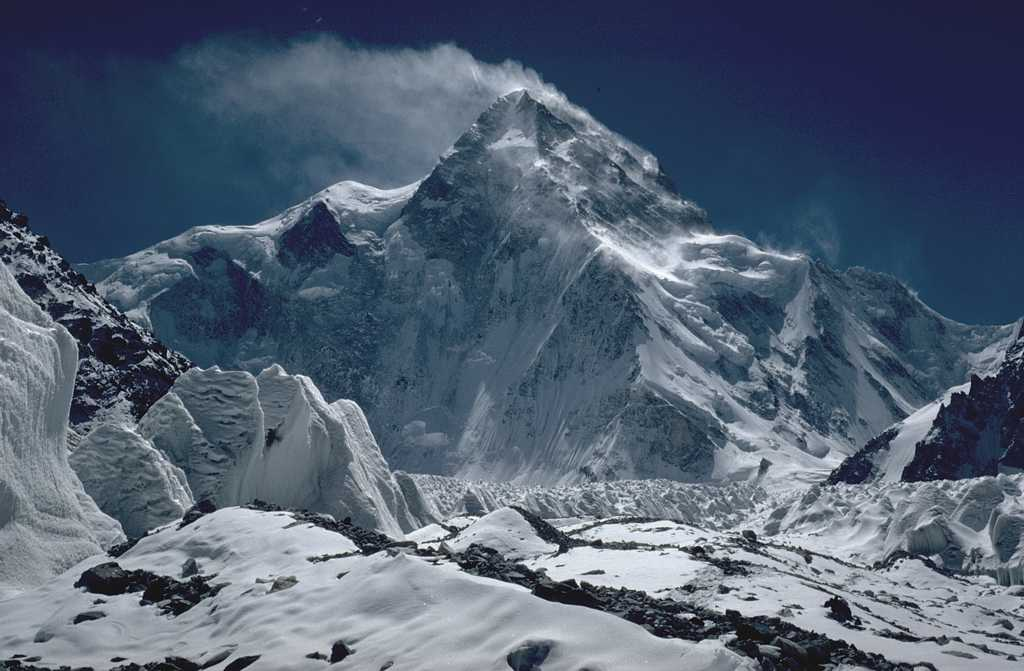
\includegraphics[height=10mm]{k2.jpg}
  \caption{The K2 mountain in Baltistan}
\end{figure}

The image below sets the height to be 30mm and the width to be 130mm. This stretches the image:
\begin{figure}[H]
  \centering
  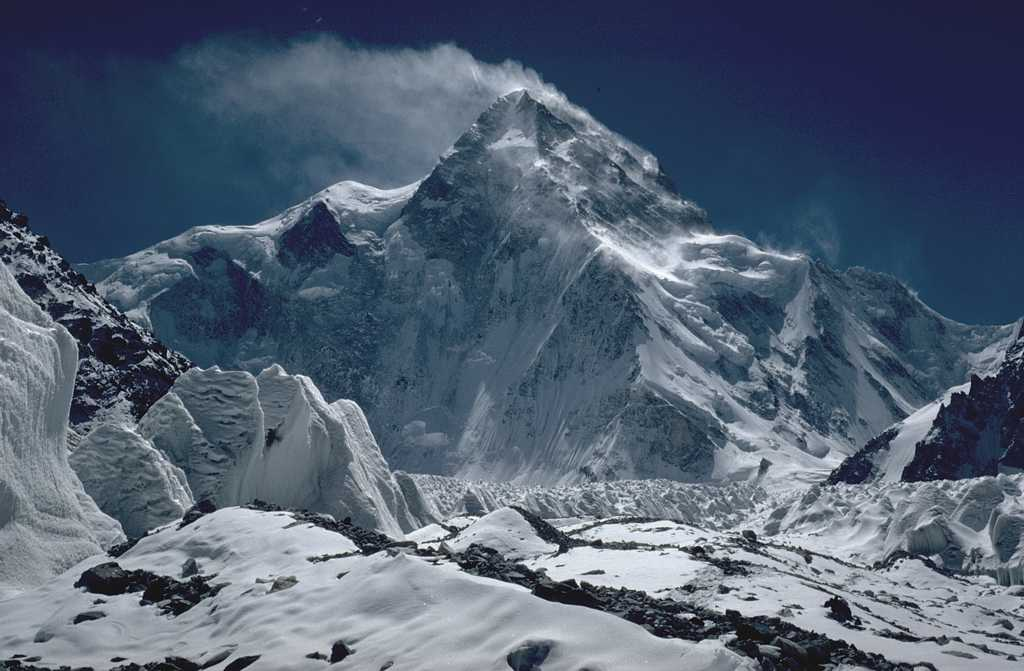
\includegraphics[height=30mm,width=130mm]{k2.jpg}
  \caption{The K2 mountain in Baltistan}
\end{figure}

\end{document}
